\documentclass{beamer}
\usetheme{Madrid}
\usepackage{lmodern}% http://ctan.org/pkg/lm
\setbeamersize{text margin left = 2.5em}
\setbeamersize{text margin right = 2.5em}
\usepackage{color}
\usepackage{graphicx}
\usepackage{MnSymbol}
\usepackage{amsmath}
\usepackage{comment}
\usepackage{tikz}
\usepackage{subfigure}
\usepackage{listings}
\usetikzlibrary{automata}

%\usepackage[backend=bibtex,sorting=none]{biblatex}
%\addbibresource{E:/Papers/LiuLab} %BibTeX�����ļ���λ��
%\setbeamerfont{footnote}{size=\tiny}
\setbeamertemplate{theorems}[numbered]
\setbeamertemplate{caption}[numbered]
%% ʹ�ý�ע���õ�Ƭijҳ���Ӳο����ס�
%% ��������ʹ�ã�\footfullcite{bib_item} %����item
%% \usepackage{anyfontsize}%% allowing font sizes at arbitrary sizes
\logo{
\includegraphics[height=0.05\textwidth]{Pic/logo}}
\newtheorem{df}{Definition}
\newtheorem{DF}{DEFINITION}
\newtheorem{prop}{Proposition}
\newtheorem{thm}{Theorem}
\newtheorem{cor}{COROLLARY}
\newtheorem{lm}{LEMMA}
% ----------------------------------------------------------------------------------------
% TITLE PAGE
% ----------------------------------------------------------------------------------------

\title{P01 Pacman}
% The short title appears at the bottom of every slide, the full title is only on the title page

\author{Suixin Ou} % Your name
\institute[SYSU] % Your institution as it will appear on the bottom of every slide, may be shorthand to save space
{
  School of Computer Science\\
  Sun Yat-sen University \\ % Your institution for the title page
  \medskip
  % Your email address
}

\date{September 14, 2021} % Date, can be changed to a custom date

\AtBeginSection[]
{
  \begin{frame}
    \tableofcontents[currentsection,currentsubsection]
  \end{frame}
}

\begin{document}

\begin{frame}
  \titlepage
\end{frame}

\begin{frame}
  \frametitle{Pacman}
    Pacman is a maze action game developed and released by Namco for arcades in 1980. The player controls the pacman through an enclosed maze. The objective of the game is to eat all of the dots placed in the maze while avoiding four colored ghosts (You can run "python pacman.py" to play the game). You need to design a Pacman agent to play the game automatically in this project.
    \begin{figure}[ht]
      \centering
      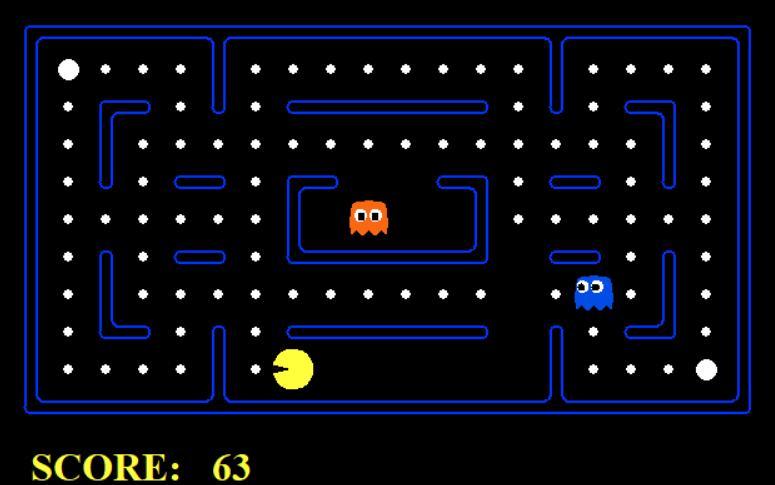
\includegraphics[width=0.68\textwidth]{Pic/pacman}
    \end{figure}
\end{frame}

\begin{frame}
  \frametitle{Part 1}
  \begin{block}{Problem}
    In this part, your Pacman agent will find paths through its maze world, both to reach a particular location and to collect food efficiently. You will build general search algorithms and apply them to Pacman scenarios.
    \begin{figure}[ht]
      \centering
      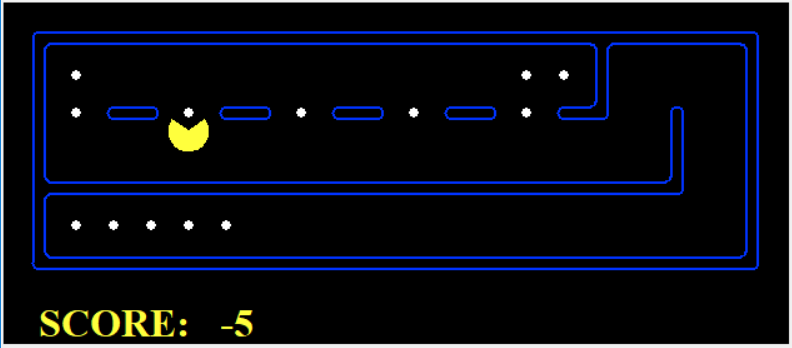
\includegraphics[width=0.7\textwidth]{Pic/part1}
      \caption{Searching by A*}
    \end{figure}
  \end{block}
\end{frame}

\begin{frame}
  \frametitle{Part 1}
  \begin{block}{Question 1 (3 points)}
    Find a path through a maze to a fixed position using the Manhattan distance heuristic. Run \begin{scriptsize}\texttt{python pacman.py -l bigMaze -z .5 -p SearchAgent -a fn=astar,heuristic=manhattanHeuristic}\end{scriptsize} for a test.
    \begin{figure}[ht]
      \centering
      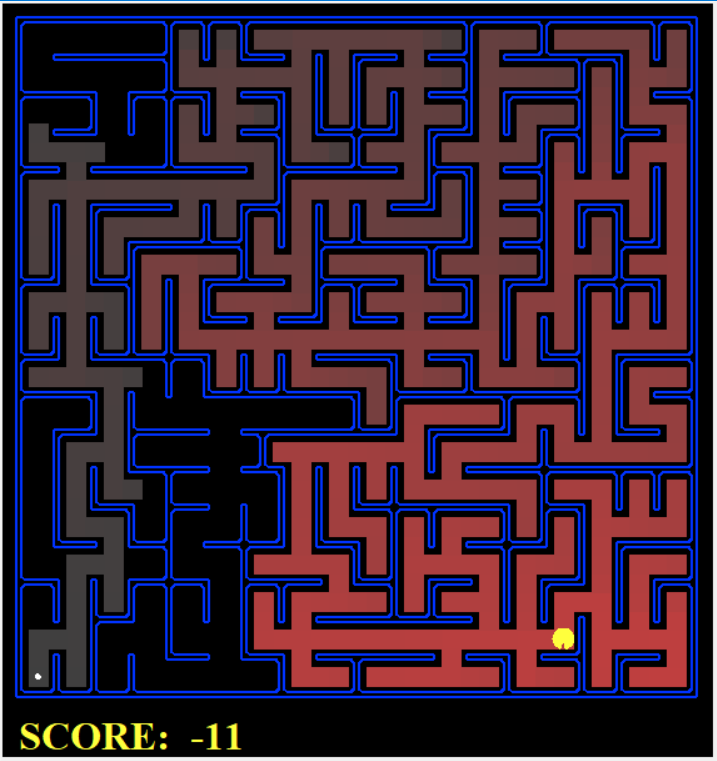
\includegraphics[width=0.35\textwidth]{Pic/q1}
      \caption{Finding a path by A*}
    \end{figure}
  \end{block}
\end{frame}


\begin{frame}
  \frametitle{Part 1}
      Given the class Position Problem
      
      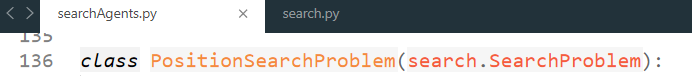
\includegraphics[width=0.7\textwidth]{Pic/posprob}

      Get initial state by problem.getStartState()
      
      
\includegraphics[width=0.43\textwidth]{Pic/getss}
      
      Get successors by problem.getSuccessors(), each successor is a tuple (nextState, action, cost)
      
      
\includegraphics[width=0.5\textwidth]{Pic/getnext}
    
      Judge that the terminate state has been reached by problem.isGoalState()
      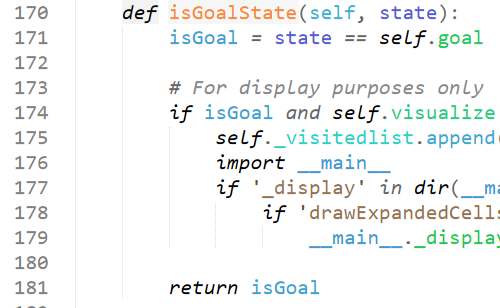
\includegraphics[width=0.48\textwidth]{Pic/isgoal}

\end{frame}

\begin{frame}

      Given Manhattan Heuristic

      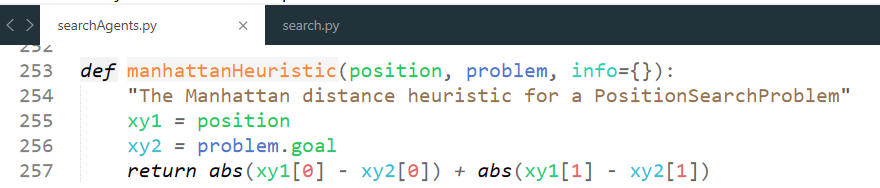
\includegraphics[width=0.8\textwidth]{Pic/manhattanHeuristic}

      \textbf{You should finish the function "aStarSearch" in search.py}

	  
      \includegraphics[width=0.95\textwidth]{Pic/AStar}
\end{frame}


\begin{frame}
  \frametitle{Part 1}
  \begin{block}{Question 2 (3 points)}
    Implement a non-trivial, consistent heuristic for the CornersProblem in cornersHeuristic. Run \begin{scriptsize}\texttt{python pacman.py -l mediumCorners -p AStarCornersAgent -z 0.5}\end{scriptsize} for a test.
    \begin{figure}[ht]
      \centering
      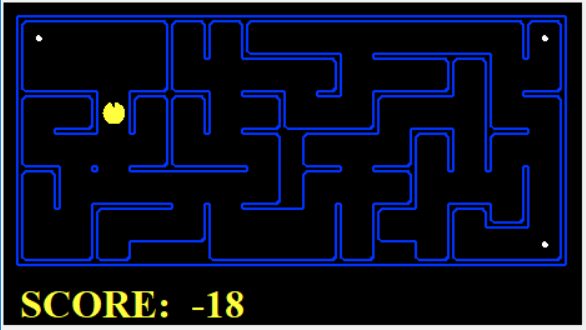
\includegraphics[width=0.6\textwidth]{Pic/q2}
      \caption{Testing Corners Heuristic}
    \end{figure}
  \end{block}
\end{frame}

\begin{frame}
  \frametitle{Part 1}

      \textbf{You should finish the class "CornersProblem" and the function "cornersHeuristic" in searchAgent.py}

      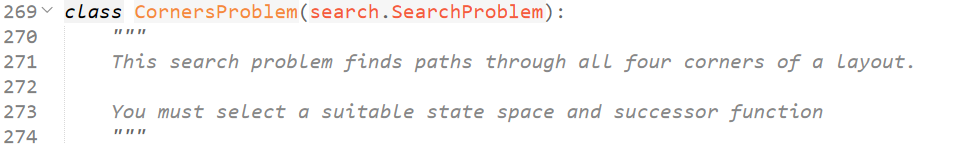
\includegraphics[width=0.8\textwidth]{Pic/cornerprob}

      Compared with the Position Problem, the status of CornersProblem should also include the four corners.

      
\includegraphics[width=0.8\textwidth]{Pic/cornerh}

	  The heuristic value can be the farthest distance from the current position to the four corners.
\end{frame}

\begin{frame}
  \begin{block}{Grading for Question 2}
Depending on how few nodes your heuristic expands, you'll be graded:

\begin{center}

\begin{tabular}{||l||l||}
  \hline\hline
  Number of nodes expanded & Grade\\
  \hline\hline
  more than 2000 & 0/3\\
  \hline\hline
  at most 2000 & 1/3\\
  \hline\hline
  at most 1600 & 2/3\\
  \hline\hline
  at most 1200 & 3/3\\
  \hline\hline
\end{tabular}
\end{center}
\end{block}
\end{frame}


\begin{frame}
  \frametitle{Part 1}
  \begin{block}{Question 3 (4 points)}
    Now we'll solve a hard search problem: eating all the Pacman food in as few steps as possible. Run \begin{scriptsize}\texttt{python pacman.py -l trickySearch -p AStarFoodSearchAgent}\end{scriptsize} for a test.
    \begin{figure}[ht]
      \centering
      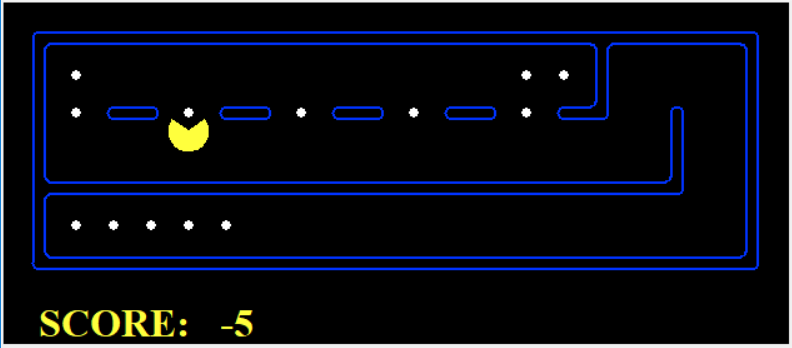
\includegraphics[width=0.6\textwidth]{Pic/part1}
      \caption{Testing Food Heuristic}
    \end{figure}
  \end{block}
\end{frame}


\begin{frame}
  \frametitle{Part 1}

      \textbf{You should finish the function "foodHeuristic" in searchAgent.py}

      
\includegraphics[width=0.7\textwidth]{Pic/fh}

  \begin{block}{Grading for Question 3}
 Depending on how few nodes your heuristic expands, you'll get additional points:

\begin{center}
\begin{tabular}{||l||l||}
  \hline\hline
  Number of nodes expanded & Grade\\
  \hline\hline
  more than 15000 & 1/4\\
  \hline\hline
  at most 15000 & 2/4\\
  \hline\hline
  at most 12000 & 3/4\\
  \hline\hline
  at most 9000 & 4/4 (full credit; medium)\\
  \hline\hline
  at most 7000 & 5/4 (optional extra credit; hard)\\
  \hline\hline
\end{tabular}
\end{center}

\end{block}


\end{frame}

\begin{frame}
  \frametitle{Part 2}
  \begin{block}{Problem}
    In this section, you will design agents for the classic version of Pacman, including ghosts. Along the way, you will implement both minimax and $\alpha-\beta$ pruning.
    \begin{figure}[ht]
      \centering
      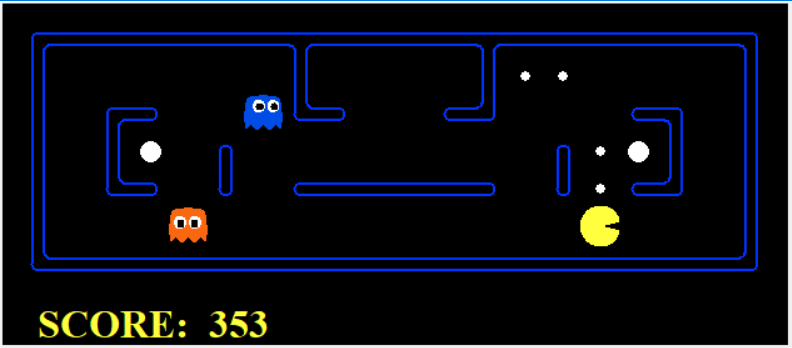
\includegraphics[width=0.7\textwidth]{Pic/part2}
      \caption{Searching by $\alpha-\beta$ pruning}
    \end{figure}
  \end{block}
\end{frame}


\begin{frame}
  \frametitle{Pacman}
  \begin{block}{Submission}

    Pack your report \texttt{report.pdf} and source code into zip file \texttt{E02\_YourNumber.zip}, then send it to \texttt{ai\_course2021@163.com}.
  \end{block}
\end{frame}




%-----------------------------------------------------------------------------------------

\begin{frame}
  \Huge{\centerline{The End}}
\end{frame}

% ----------------------------------------------------------------------------------------


\end{document}
